\begin{frame}
    \titlepage
\end{frame}

\begin{frame}{last time: VMs}
    \begin{itemize}
    \item \myemph{configurablity}
        \begin{itemize}
        \item consistent environment
        \end{itemize}
    \item \myemph{isolation}
        \begin{itemize}
        \item run malware in safe environment
        \end{itemize}
    \item key mechanism: hardware support
        \begin{itemize}
        \item hardware gives VM monitor control when needed
        \end{itemize}
    \item backup mechanism: emulation, binary translation
    \end{itemize}
\end{frame}

\begin{frame}{from last time: POPF}
    \begin{itemize}
    \item on POPF
    \vspace{.5cm}
    \item user mode: \myemph{silently} doesn't change \\ interrupt enable flag ({\tt IF})
        \begin{itemize}
        \item (and some other ``privileged'' flags)
        \end{itemize}
    \item kernel mode: does change {\tt IF}
    \item what VM wants:
        \begin{itemize}
        \item call VM monitor to change \myemph{simulated} {\tt IF}
        \end{itemize}
    \end{itemize}
\end{frame}

\begin{frame}{from last time: the VM stack}
    \begin{itemize}
    \item guest OS machine code runs on \myemph{real hardware}
    \item ``normal'' instructions:
        \begin{itemize}
        \item run directly on real hardware
        \end{itemize}
    \item privileged operations:
        \begin{itemize}
        \item real hardware gives control to \myemph{host} OS
        \item host OS gives control to VM monitor
        \end{itemize}
    \end{itemize}
\end{frame}

\begin{frame}{from last time: binary translation}
    \begin{itemize}
    \item key idea: machine code to new machine code
        \begin{itemize}
        \item change/translate as needed
        \end{itemize}
    \item in small segments: end by returning to translator
        \begin{itemize}
        \item avoid needing to translate whole program
        \item handle things like loading new code
        \end{itemize}
    \item efficient version:
        \begin{itemize}
        \item cache translated code
        \item replace calls to translator with jumps to translated code
        \end{itemize}
    \end{itemize}
\end{frame}

\begin{frame}[fragile,label=binTransIdea]{binary translation idea}
\lstset{
    language=myasm,
    style=small,
    morekeywords={movq,addss,subss}
}
\begin{tikzpicture}
\tikzset{
    code/.style={inner sep=0mm,align=left},
    hiOn/.style={alt=#1{rounded corners,fill=green,fill opacity=0.3,text opacity=1.0}{}},
    markOn/.style={alt=#1{rounded corners,draw,thick}{}},
}
\node[code,markOn=<2>,hiOn=<3>] (bb1) {
\begin{lstlisting}
0x40FE00: addq %rax, %rbx
movq 14(%r14,4), %rdx
addss %xmm0, (%rdx)
...
0x40FE3A: jne 0x40F404
\end{lstlisting}
};
\node[right=.25cm of bb1,visible on=<2>,align=left] {
    divide machine code \\
    into \textit{basic blocks} \\
    (= ``straight-line'' code) \\
    (= code till \\ 
    jump/call/etc.)
};
\node[code,right=.25cm of bb1,visible on=<3>] (bb1New) {
generated code: \\
\begin{lstlisting}
// addq %rax, %rbx
movq rax_location, %rdi
movq rbx_location, %rsi
call checked_addq
movq %rax, rax_location
...
// jne 0x40F404
... // get CCs 
je do_jne
movq $0x40FE3F, %rdi
jmp translate_and_run
do_jne:
movq $0x40F404, %rdi
jmp translate_and_run
\end{lstlisting}
};
\node[code,markOn=<2>,anchor=north west] (bb2) at (bb1.south west){
\begin{lstlisting}
subss %xmm0, 4(%rdx)
...
je 0x40F543
\end{lstlisting}
};
\node[code,markOn=<2>,anchor=north west] (bb3) at (bb2.south west){
\begin{lstlisting}
ret
\end{lstlisting}
};
\end{tikzpicture}
\end{frame}

\lstset{language=myasm}

\section{definitive sources}

\begin{frame}{x86-64 assembly}
    \begin{itemize}
    \item your assignments will use it
    \item will have examples with lots of assembly
    \item x86-64 machine code will come up
    \end{itemize}
\end{frame}

\begin{frame}{x86-64 assembly}
\begin{itemize}
\item history: AMD constructed 64-bit extension to x86 first
    \begin{itemize}
    \item marketing term: AMD64
    \end{itemize}
\item Intel first tried a new ISA (Itanium), which failed
\item Then Intel copied AMD64
    \begin{itemize}
    \item marketing term: EM64T
        \begin{itemize}\item Extended Memory 64 Technology\end{itemize}
    \item later marketing term: Intel 64
    \end{itemize}
\item both Intel and AMD have manuals --- definitive reference
\end{itemize}
\end{frame}

\begin{frame}

\includegraphics[height=0.9\textheight]{manual-screenshot}
\end{frame}

\begin{frame}{x86-64 manuals}
\begin{itemize}
\item Intel manuals:
    \begin{itemize}
    \item \small \url{https://software.intel.com/en-us/articles/intel-sdm}
    \item 24 MB, 4684 pages
    \item Volume 2: instruction set reference (2190 pages)
    \end{itemize}
\item AMD manuals:
    \begin{itemize}
    \item \small \url{https://support.amd.com/en-us/search/tech-docs}
    \item ``AMD64 Architecture Programmer's Manual''
    \end{itemize}
\end{itemize}
\end{frame}

\begin{frame}{example manual page}
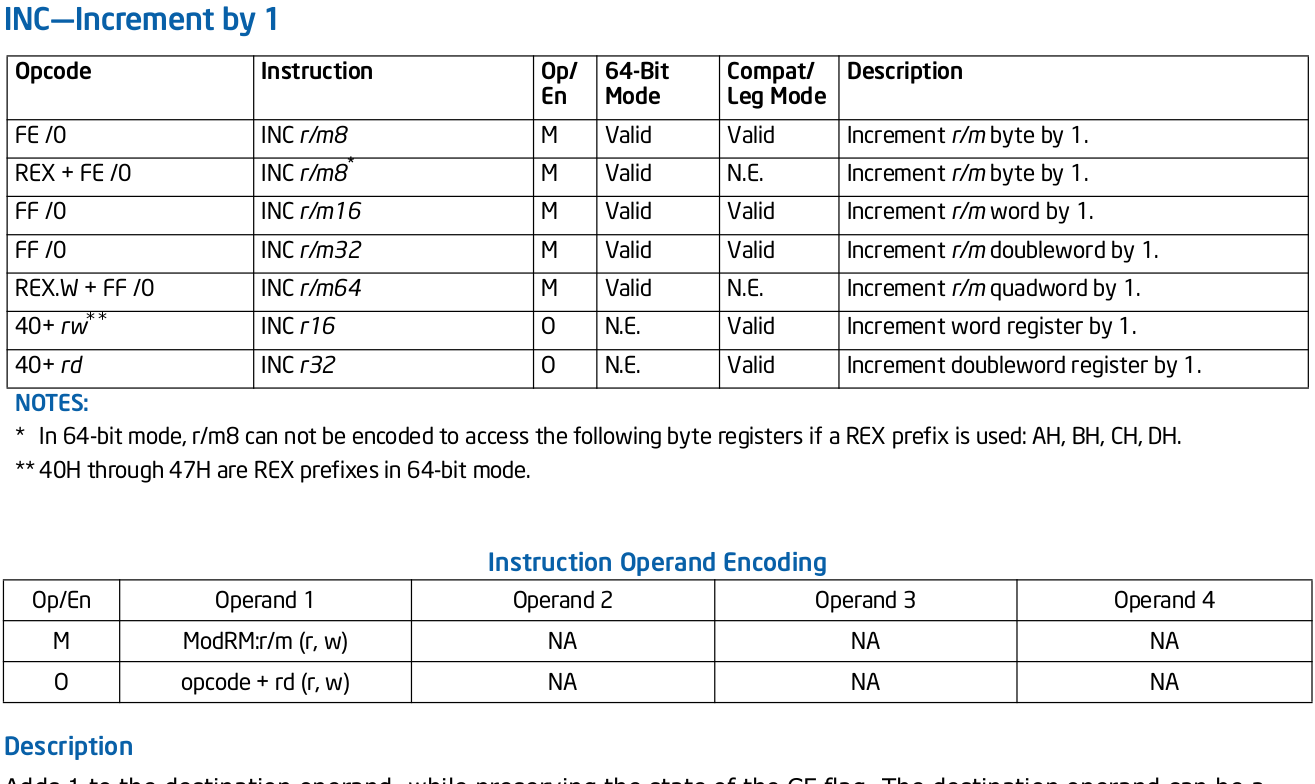
\includegraphics[width=\textwidth]{example-manual}
\end{frame}

\begin{frame}{instruction listing parts (1)}
    \begin{itemize}
    \item opcode --- first part of instruction encoding
        \begin{itemize}
        \item yes, variable length
        \item ``REX''???
        \item more later (today or next week)
        \end{itemize}
    \item instruction --- Intel assembly skeleton
    \item {\tt r/m32} --- 32-bit memory or register value
    \item 64-bit mode --- does instruction exist in 64-bit mode?
    \item compat/leg mode --- in 16-bit/32-bit modes?
    \end{itemize}
\end{frame}

\begin{frame}{instruction listing parts (2)}
    \begin{itemize}
    \item dscription + operation (later on page)
        \begin{itemize}
        \item text and pseudocode description
        \end{itemize}
    \item flags affected
        \begin{itemize}
        \item flags --- used by {\tt jne}, etc.
        \end{itemize}
    \item exceptions --- how can OS be called from this?
        \begin{itemize}
        \item example: can invalid memory access happen?
        \end{itemize}
    \end{itemize}
\end{frame}

\begin{frame}{recall: x86-64 general purpose registers}
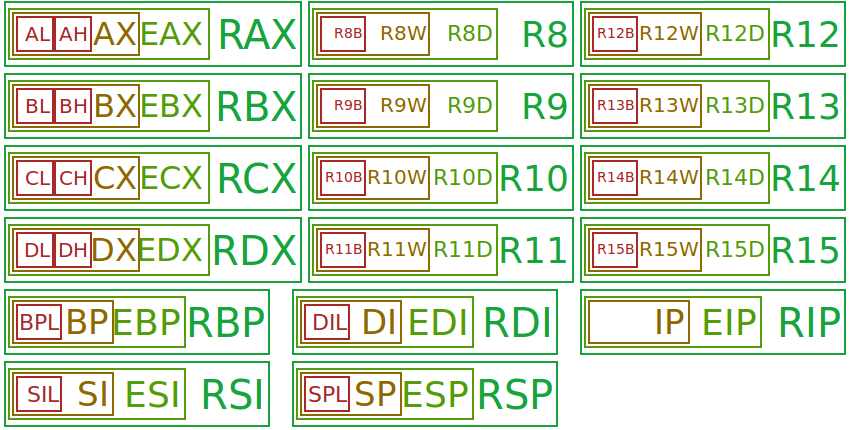
\includegraphics[width=\textwidth]{x86-gprs}
\imagecredit{Immae via Wikipedia}
\end{frame}

\begin{frame}[fragile,label=overlap]{overlapping registers (1)}
\begin{itemize}
\item setting 32-bit registers sets \myemph{whole} 64-bit register
\item extra bits are always zeroes
\end{itemize}
\begin{lstlisting}[style=small]
movq $0x123456789abcdef, %rax
xor %eax, %eax
// %rax is 0, not 0x1234567800000000
movl $-1, %ebx
// %rbx is 0xFFFFFFFF, not -1 (0xFFFFF...FFF)
\end{lstlisting}
\end{frame}

\begin{frame}[fragile,label=overlap2]{overlapping registers (2)}
\begin{itemize}
\item setting \myemph{8/16-bit registers} doesn't change rest of 64-bit register:
\end{itemize}
\begin{lstlisting}[style=small]
movq $0x12345789abcdef, %rax
movw $0xaaaa, %ax
// %rax is 0x123456789abaaaa
\end{lstlisting}
\end{frame}

% FIXME: manual screenshots

\section{AT\&T versus Intel}

\begin{frame}{AT\&T versus Intel syntax}
    \begin{itemize}
    \item AT\&T syntax: \\ {\tt movq \$42, 100(\%rbx,\%rcx,4)}
    \item Intel syntax: \\ {\tt mov QWORD PTR [rbx+rcx*4+100], 42}
    \item effect (pseudo-C): \\ {\tt memory[rbx + rcx * 4 + 100] <- 42}
    \end{itemize}
\end{frame}

\begin{frame}[fragile,label=att1]{AT\&T syntax (1)}
\begin{lstlisting}
movq $42, 100(%rbx,%rcx,4)
\end{lstlisting}
    \begin{itemize}
    \item destination \myemph{last}
    \item constants start with {\tt \$}
    \item registers start with {\tt \%}
    \end{itemize}
\end{frame}

\begin{frame}[fragile,label=att2]{AT\&T syntax (2)}
\begin{lstlisting}
movq $42, 100(%rbx,%rcx,4)
\end{lstlisting}
    \begin{itemize}
    \item operand length: {\tt q}
        \begin{itemize}
        \item {\tt l} = 4; {\tt w} = 2; {\tt b} = 1
        \item 
        \end{itemize}
    \item {\tt 100(\%rbx,\%rcx,4)}: \\ {\tt memory[100 + rbx + rcx * 4]}
    \item {\tt sub \%rax, \%rbx}: {\tt rbx $\leftarrow$ rbx - rax}
    \end{itemize}
\end{frame}

\begin{frame}{Intel syntax}
    \begin{itemize}
    \item destination \myemph{first}
    \item {\tt [...]} indicates location in memory
    \item {\tt QWORD PTR [...]} for 8 bytes in memory
        \begin{itemize}
        \item DWORD for 4
        \item WORD for 2
        \item BYTE for 1
        \end{itemize}
    \end{itemize}
\end{frame}

% FIXME: move this?
\begin{frame}[fragile,label=LEA]{On LEA}
    \begin{itemize}
    \item LEA = Load Effective Address
    \item uses the syntax of a memory access, but\ldots{}
    \item just computes the address and uses it:
    \item {}\lstinline|leaq 4(%rax), %rax| same as \lstinline|addq $4, %rax|
        \begin{itemize}
        \item almost --- doesn't set condition codes
        \end{itemize}
    \end{itemize}
\end{frame}

\begin{frame}[fragile,label=LEATricks]{LEA tricks}
    \begin{itemize}
    \item {}\lstinline|leaq (%rax,%rax,4), %rax| multiplies {\tt \%rax} by 5
        \begin{itemize}
        \item {\tt address-of(memory[rax + rax * 4])}
        \end{itemize}
    \item {}\lstinline|leal (%rbx,%rcx), %eax| adds rbx + rcx into eax
        \begin{itemize}
        \item ignores top 64-bits
        \end{itemize}
    \end{itemize}
\end{frame}

\begin{frame}[fragile,label=question]{question}
\lstset{style=small,language=myasm}
\begin{lstlisting}
.data
string:
    .asciz "abcdefgh"
.text
    movq $string, %rax
    movq string, %rdx
    movb (%rax), %bl
    leal 1(%rbx), %ebx
    movb %bl, (%rax)
    movq %rdx, 4(%rax)
\end{lstlisting}
{\small What is the final value of string?}
\begin{tabular}{ll}
a. "abcdabcd" & d. "abcdefgh" \\
b. "bbcdefgh" & e. something else / not enough info \\
c. "bbcdabcd" & ~ \\
\end{tabular}
\end{frame}

\section{x86-64 calling conventions}

\begin{frame}{Linux x86-64 calling convention}
    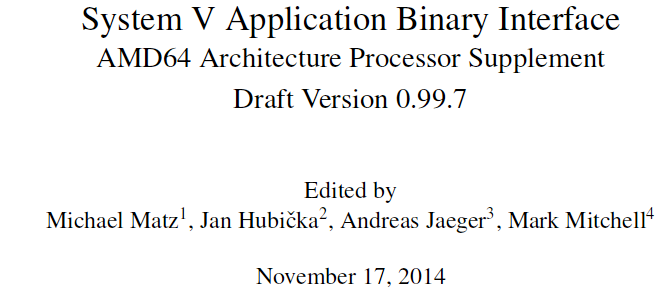
\includegraphics[width=\textwidth]{sysv-abi-front}
\end{frame}

\begin{frame}{Linux x86-64 calling summary}
\begin{itemize}
    \item first 6 arguments: \%rdi, \%rsi, \%rdx, \%rcx, \%r8, \%r9
    \item additional arguments: push on stack
    \item return address: push on stack
        \begin{itemize}
        \item {\tt call}, {\tt ret} instructions assume this
        \end{itemize}
    \item return value: \%rax
\end{itemize}
\end{frame}

\begin{frame}{caller-saved registers}
    \begin{itemize}
        \item functions \myemph{may} freely \myemph{trash} these
        \vspace{.5cm}
        \item return value register {\tt \%rax}
        \item argument registers: \\
            \begin{itemize}
            \item {\tt \%rdi}, {\tt \%rsi}, {\tt \%rdx}, 
              {\tt \%rcx}, {\tt \%r8}, {\tt \%r9}
              \end{itemize}
        \item \%r11
        \item MMX/SSE/AVX registers: {\tt \%xmm0-15}, etc.
        \item floating point stack: {\tt \%st(0)-\%st(7)}
        \item condition codes (used by {\tt jne}, etc.)
    \end{itemize}
\end{frame}

\begin{frame}[fragile,label=calleeSaved]{callee-saved registers}
    \begin{itemize}
    \item functions \myemph{must preserve} these
    \vspace{.5cm}
    \item {\tt \%rsp} (stack pointer), {\tt \%rbp} (frame pointer, maybe)
    \item {\tt \%r12-\%r15}
    \end{itemize}
\end{frame}

\begin{frame}[fragile,label=callerCallee]{caller/callee-saved}
\lstset{style=small}
\begin{lstlisting}
foo:
    pushq %r12 // r12 is caller-saved
    ... use r12 ...
    popq %r12
    ret

...
other_function:
    pushq %r11 // r11 is caller-saved
    ...
    callq foo
    popq %r11
\end{lstlisting}
\end{frame}

% XXX enter/leave ???

\subsection{the call stack}

\begin{frame}[fragile,label=callStack]{the call stack}
\begin{lstlisting}[language=C,style=small]
foo(a,b,c,d,e,f,g,h);
\end{lstlisting}
\begin{tikzpicture}
\tikzset{>=Latex}
\matrix[tight matrix,nodes={text width=7cm,font=\tt}] (theStack) {
    \ldots \\
    \normalfont (stack allocations in caller) \\
    \normalfont (saved registers, if any) \\
    h \\
    g \\
    \normalfont return address \\
    \normalfont (first stack allocation in {\tt foo}) \\
    \ldots \\
};
\draw[very thick,->] ([xshift=0.25cm]theStack-1-1.east)  -- ([xshift=0.25cm]theStack-8-1.east)
    node[right] {decreasing addresses};
\draw[red,thick,->] (theStack-6-1.east) -- ++(.5cm,0cm) node[right] {stack pointer after call};
\end{tikzpicture}
\end{frame}

\begin{frame}[fragile,label=conventionEx]{calling convention example}
\begin{lstlisting}[language=C,style=small]
int foo(int a, int b, int c, int d, int e, int f, int g, int h);
...
foo(1, 2, 3, 4, 5, 6, 7, 8);
\end{lstlisting}
\begin{lstlisting}[language=myasm,style=small]
pushq   $8
pushq   $7
movl    $6, %r9d
movl    $5, %r8d
movl    $4, %ecx
movl    $3, %edx
movl    $2, %esi
movl    $1, %edi
call    foo
/* return value in %eax */
\end{lstlisting}
\end{frame}

\section{x86-64 floating point}

\subsection{x87 versus SSE2}

\begin{frame}{floating point operations}
    \begin{itemize}
    \item x86 has two ways to do floating point
    \item method one --- legacy: x87 floating point instructions
        \begin{itemize}
        \item still common in 32-bit x86
        \end{itemize}
    \item method two --- SSE instructions
        \begin{itemize}
        \item work more like what you expect
        \end{itemize}
    \end{itemize}
\end{frame}

\begin{frame}[fragile,label=x87Stack]{x87 floating point stack}
    \begin{itemize}
    \item x87: 8 floating point registers
        \begin{itemize}
        \item {\tt \%st(0)} through {\tt \%st(7)}
        \end{itemize}
    \item arranged as a \myemph{stack of registers}
    \item example: \lstinline|fld 0(%rbx)| 
        \begin{tabular}{l@{: }ll}
        ~ & before & after \\
        {\tt st(0)} & 5.0 & (value from memory at {\tt \%rbx}) \\
        {\tt st(1)} & 6.0 & 5.0 \\
        {\tt st(1)} & 7.0 & 6.0 \\
        \ldots      & \ldots & \ldots \\
        {\tt st(6)} & 10.0 & 9.0 \\
        {\tt st(7)} & 11.0 & 10.0 \\
        \end{tabular}
    \end{itemize}
\end{frame}

\begin{frame}{x87}
    \begin{itemize}
    \item not going to talk about x87 more in this course
    \item essentially obsolete with 64-bit x86
    \end{itemize}
\end{frame}

\begin{frame}[fragile,label=sseRegs]{SSE registers}
    \begin{itemize}
    \item SSE and SSE2 extensions brought \myemph{vector instructions}
    \end{itemize}
\lstset{
    language=myasm,
    style=small,
    moredelim={**[is][\btHL<2|handout:0>]{&2}{&}},
    moredelim={**[is][\btHL<3|handout:0>]{&3}{&}},
    moredelim={**[is][\btHL<4|handout:0>]{&4}{&}},
    morekeywords={.float,movps,addps},
}
\begin{lstlisting}
&2numbers: .float 1 .float 2 .float 3. float 4&
ones:    .float 1 .float 3 .float 5 .float 7
result:  .float 0 .float 0 .float 0 .float 0
...
&3movps& numbers, %xmm0
movps ones, %xmm1
&4addps& %xmm1, %xmm0
movps %xmm0, result
/* result contains: 1+1=2,2+3=5,3+5=8,4+7=11 */
\end{lstlisting}
\begin{tikzpicture}[overlay,remember picture]
    \coordinate (overlayPlace) at ([xshift=1cm,yshift=-1cm]current page.center);
    \tikzset{overThing/.style={
        draw=red,very thick,rectangle,at=(overlayPlace),
        anchor=west,align=left
    }}
    \begin{visibleenv}<2|handout:0>
        \node [overThing] {array of 4 floats};
    \end{visibleenv}
    \begin{visibleenv}<3|handout:0>
        \node [overThing] {move packed single \\ (single-precision float)};
    \end{visibleenv}
    \begin{visibleenv}<4|handout:0>
        \node [overThing] {add packed single \\ (single-precision float)};
    \end{visibleenv}
\end{tikzpicture}
\end{frame}

\begin{frame}{XMM registers}
\begin{itemize}
\item {\tt \%xmm0} through {\tt \%xmm15} {\small ({\tt \%xmm8} on 32-bit)}
\item each holds 128-bits ---
    \begin{itemize}
    \item 32-bit floating point values ({\tt addps})
    \item 64-bit floating point values ({\tt addpd}) 
    \item 64/32/16/8-bit integers ({\tt paddq/d/w/b})
    \item \myemph<2>{a 32-bit floating point value}, 96 unused bits ({\tt addss})
    \item \myemph<2>{a 64-bit floating point value}, 64 unused bits ({\tt addsd})
    \end{itemize}
\end{itemize}
\end{frame}

\begin{frame}[fragile,label=fpExample]{FP example}
\lstset{language=myasm,morekeywords={movss,mulss,subq}}
\begin{lstlisting}
multiplyEachElementOfArray:
/* %rsi = array, %rdi length,
   %xmm0 multiplier */
loop:   test %rdi, %rdi
        je done
        movss (%rsi), %xmm1
        mulss %xmm0, %xmm1
        movss %xmm1, (%rsi)
        subq $1, %rdi
        addq $4, %rsi
        jmp loop
done:   ret
\end{lstlisting}
\end{frame}

\subsection{calling convention}

\begin{frame}{floating point calling convention}
    \begin{itemize}
    \item use {\tt \%xmm} registers in order
    \end{itemize}
\end{frame}

\begin{frame}[fragile,label=variadic]{note: variadic functions}
    \begin{itemize}
    \item variable number of arguments
        \begin{itemize}
        \item {\tt printf}, {\tt scanf}, \ldots
        \item see {\tt man stdarg}
        \end{itemize}
    \vspace{.5cm}
    \item same as usual 
    \item \ldots but \lstinline|%rax| contains number of {\tt \%xmm} used
    \end{itemize}
\end{frame}

\begin{frame}{AVX}
    \begin{itemize}
    \item recent Intel/AMD processors implement the AVX extension
    \item adds {\tt \%ymm} registers
    \item 256-bit versions of {\tt \%xmm} registers
    \item XMM0 is a name for the bottom 128 bits of YMM0
        \begin{itemize}
        \item like RAX and EAX, or RDX and EDX
        \end{itemize}
    \item (later extension: even larger zmm registers)
    \end{itemize}
\end{frame}

\section{x86-64 addressing modes}

\begin{frame}[fragile,label=addressing1]{addressing modes (1)}
    \begin{itemize}
        \item {\tt \$constant}
        \item {\tt displacement(\%base, \%index, scale)}
            \begin{itemize}
            \item {\tt displacement} (absolute)
            \item {\tt displacement(\%base)}
            \item {\tt displacement(,\%index, scale)}
            \end{itemize}
        \item (= $\text{displacement} + \text{base} + \text{index} \times \text{scale}$)
    \end{itemize}
\end{frame}

\begin{frame}[fragile,label=addressing2]{addressing modes (2)}
    \begin{itemize}
        \item {\tt displacement(\%rip)} (64-bit only)
\begin{lstlisting}
thing: .quad 42
...
movq thing(%rip), %rax
\end{lstlisting}
        \begin{itemize}
        \item encoded as offset from \myemph{address of next instruction}
        \item (normally: label encoded as 32 or 64-bit address)
        \item helps \myemph{relocatable code}
        \end{itemize}
    \end{itemize}
\end{frame}

\begin{frame}[fragile,label=addressing3]{addressing modes (3)}
    \begin{itemize}
        \item {\tt jmp *\%rax} (or {\tt call})
        \begin{itemize}
        \item Intel syntax: {\tt jmp RAX}
        \item what you'd expect to be {\tt jmp (\%rax)}
        \end{itemize}
        \item {\tt jmp *(\%rax)}
        \begin{itemize}
        \item read value from memory at RAX
        \item PC becomes location in that value
        \item Intel syntax: {\tt jmp [RAX]}
        \end{itemize}
        \item {\tt jmp *(\%rax,\%rbx,8)}
    \end{itemize}
\end{frame}

\section{segmentation}

\begin{frame}[fragile,label=vm]{recall(?): virtual memory}
\begin{itemize}
\item illuision of \myemph{dedicated memory}
\end{itemize}
\begin{tikzpicture}
\tikzset{
    every node/.style={font=\small},
}
\node[align=center] (progAAddr) {Program A \\ addresses};
\node[below=1cm of progAAddr,align=center] (progBAddr) {Program B \\ addresses};
\node[draw, right=1cm of progAAddr,align=center] (translationA) { mapping \\ (set by OS) };
\node[draw, right=1cm of progBAddr,align=center] (translationB) { mapping \\ (set by OS) };
\node[draw,rectangle split, rectangle split parts=6, anchor=north west,label={north:real memory}] (mem) at ([xshift=1cm]translationA.north east) {
    \nodepart{one}
    Program A code 
    \nodepart{two}
    Program B code
    \nodepart{three}
    Program A data
    \nodepart{four}
    Program B data
    \nodepart{five}
    OS data
    \nodepart{six}
    \ldots
};
\draw[-Latex,green,thick] (progAAddr) -- (translationA) (translationA.east) -- (mem.one west);
\draw[-Latex,green,thick] (translationA.east) -- (mem.three west);
\draw[-Latex,blue,thick] (progBAddr) -- (translationB) (translationB.east) -- (mem.two west);
\draw[-Latex,blue,thick] (translationB.east) -- (mem.four west);
\node[thick,red,draw,anchor=north west] (error) at ([yshift=-.5cm]mem.south west) {trigger error};
\draw[-Latex,green,thick] (translationA.east) -- (error.west);
\draw[-Latex,blue,thick] (translationB.east) -- (error.west);
\draw[-Latex,green,ultra thick,dotted] (translationA.east) -- (mem.five west);
\draw[-Latex,blue,ultra thick,dotted] (translationB.east) -- (mem.five west);
\draw[-Latex,ultra thick,dotted] ([xshift=-3cm,yshift=-.5cm]translationB.south) -- ([xshift=-2cm,yshift=-.5cm]translationB.south)
    node[right] {= kernel-mode only};
\end{tikzpicture}
\end{frame}

\begin{frame}[fragile,label=segmentation]{segmentation}
    \begin{itemize}
    \item before virtual memory, there was \myemph{segmentation}
    \end{itemize}
\begin{tikzpicture}
    \tikzset{>=Latex}
    \node[draw,label={north:address},rectangle split,rectangle split parts=2,
        rectangle split horizontal,font=\small,align=left] (address) {
        segment \#: \\ \color{orange!70!black}{\tt 0x1} \nodepart{two} offset: \\ \color{magenta!70!black}{\tt 0x23456}
    };
    \matrix[tight matrix,nodes={text width=2cm,font=\small\tt,text depth=.4ex,text height=1.2ex},
        column 3/.style={font=\scriptsize\normalfont},
        anchor=north west
    ] (table) at ([xshift=.5cm]address.north east){
        seg \# \& base \& limit \\
        0 \& 0x14300 \& 0x60000 \\
        |[orange!70!black]| 1 \& |[blue!70!black]| 0x50000 \& |[green!70!black]| 0x6F000 \\
        2 \& 0x70000 \& 0x30000 \\
    };
    \node[draw,circle,font=\large] (plus) at ([yshift=-2cm]address.two south) { $+$ };
    \node[font=\large,draw] (less) at (table-3-3.south |- plus) { $<=$ };
    \draw[magenta!70!black,thick,->] (address.two south) -- (plus);
    \draw[blue!70!black,thick,->] (table-3-2.south) |- (plus);
    \draw[green!70!black,thick,->] ([xshift=.25cm]table-3-3.south) -- ([xshift=.25cm]less.north);
    \draw[magenta!70!black,thick,->] (address.two south) -- ($(plus.north) + (0, .5cm)$) -| ([xshift=-.25cm]less.north);
    \draw[thick,->] (plus) -- ++ (0,-1cm) node[below] { computed address };
    \draw[thick,->] (less) -- ++ (0,-1cm) node[below,align=center] { no segmentation \\ fault?};
\end{tikzpicture}
\end{frame}

\begin{frame}[fragile, label=x86Seg]{x86 segmentation}
\begin{itemize}
\item addresses you've seen are the \myemph{offsets}
\item but every access uses a segment number!
\item segment numbers come from registers
    \begin{itemize}
    \item CS --- code segment number (jump, call, etc.)
    \item SS --- stack segment number (push, pop, etc.)
    \item DS --- data segment number (mov, add, etc.)
    \item ES, FS, GS --- extra segments (never default)
    \end{itemize}
\item instructions can have a \myemph{segment override}:
\begin{lstlisting}
movq $42, %fs:100(%rsi)
    // move 42 to segment (# in FS),
    // offset 100 + RSI 
\end{lstlisting}
\end{itemize}
\end{frame}


\begin{frame}[fragile,label=x86SegPic]
\vspace{-.25cm}
\tikzset{every picture/.style={very thick},every node/.style={fill=white,inner sep=.1mm}}
\begin{tikzpicture}
\node[anchor=north west] at (0,0){
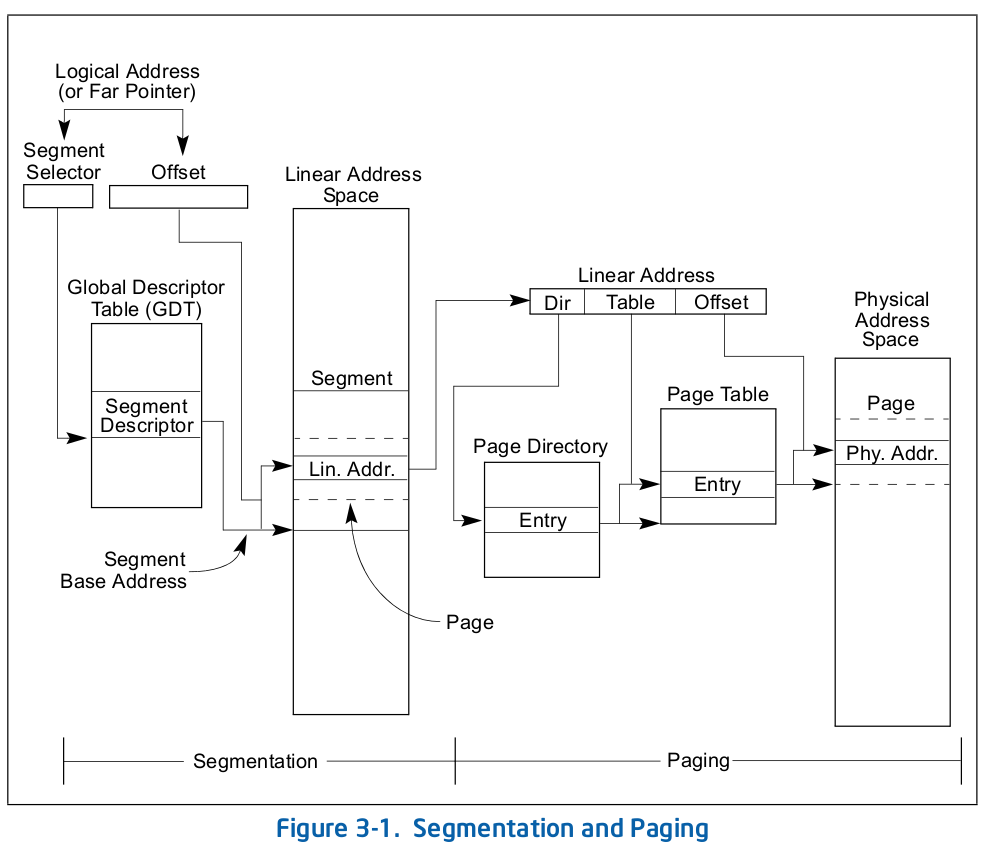
\includegraphics[width=\textwidth]{seg-and-page}
};
%\draw[help lines] (0,0) grid (12, -8);
\begin{visibleenv}<2>
    \draw[blue] (0.8,-0.8) rectangle (2.5,-1.4);
    \node[text=blue!70!black,anchor=south,font=\small] at (1.6,-.8) {program address};
    \draw[green] (6.4,-3.3) rectangle (9.1,-3.9);
    \node[text=green!70!black,anchor=south,font=\small,align=center] at (7.5,-3.3) {after segmentation \\
                                                  ``virtual address''};
    \draw[magenta] (0.9,-3.4) rectangle (2.8,-6.1);
    \node[text=magenta!70!black,anchor=south,font=\small] at (1.8,-3.4) {segment table};
\end{visibleenv}
\begin{visibleenv}<3>
    \draw[red] (0.3,-1.6) rectangle (1.4,-2.4);
    \node[text=red,anchor=west] at (1.4,-2.0) {from instruction + segment register};
\end{visibleenv}
\end{tikzpicture}
\imagecredit{Figure: Intel manuals, Vol 3A}
\end{frame}

\begin{frame}{segments and privilege levels}
    \begin{itemize}
    \item user mode/kernel mode
    \item in x86 --- controlled by segment table entry!
    \item 64 versus 32-bit mode
    \item in x86 --- controlled by segment table entry!
    \end{itemize}
\end{frame}

\begin{frame}{x86 segment descriptor}
\vspace{-.25cm}
\tikzset{every picture/.style={very thick},every node/.style={fill=white,inner sep=.2mm}}
\begin{tikzpicture}
\node[anchor=north west] at (0,0){
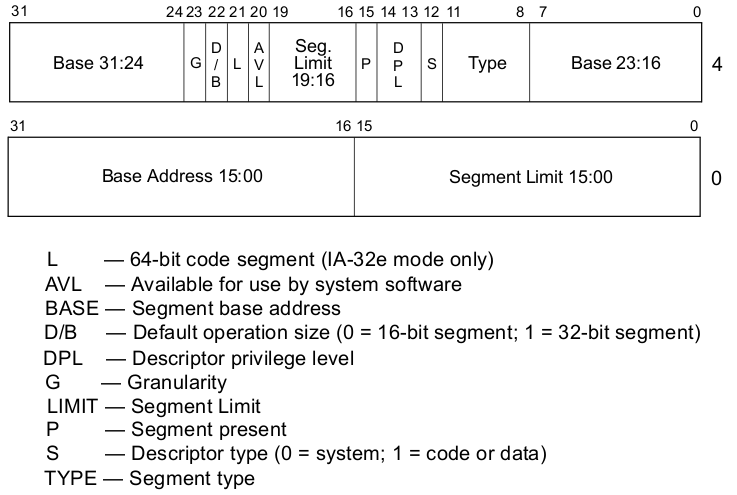
\includegraphics[width=\textwidth]{segment-descr}
};
%\draw[help lines] (0,0) grid (12, -8);
\begin{visibleenv}<2>
\draw[draw=red] (0.6, -5.4) rectangle (5.8, -5.8) node[right,text=red] {
    user or kernel mode? (if code)
};
\end{visibleenv}
\begin{visibleenv}<3>
\draw[draw=red] (0.6, -3.9) rectangle (8.0, -4.3);
\draw[draw=red] (0.6, -5.0) rectangle (11.0, -5.4);
\node[draw=red,text=red!60!black,anchor=north] at (5.0, -5.6) {
    64-bit or 32-bit or 16-bit mode? (if code)
};
\end{visibleenv}
\end{tikzpicture}
\imagecredit{Figure: Intel manuals, Volume 3A}
\end{frame}

\begin{frame}{64-bit segmentation}
\begin{itemize}
\item in 64-bit mode:
\item limits are ignored
\item base addresses are ignored
\item \ldots except for {\tt \%fs}, {\tt \%gs}
\item effectively: extra pointer register
\end{itemize}
\end{frame}

\begin{frame}{segments on x86}
\begin{itemize}
\item mostly unused even in 32-bit mode
\item exception: thread-local storage --- FS or GS acts as pointer!
\end{itemize}
\end{frame}

% FIXME: more detail on segmentation and privilege level

\section{conclusion}

\begin{frame}{reading assembly guides}
    \begin{itemize}
    \item the calling convention is your friend
        \begin{itemize}
        \item identify functions, arguments, purpose, etc.
        \end{itemize}
    \item don't be scared of the manuals
        \begin{itemize}
        \item or alternate resources
        \item if you don't know what an instruction is\ldots
        \end{itemize}
    \end{itemize}
\end{frame}

\begin{frame}{next: machine code}
    \begin{itemize}
    \item what's actually in binaries
    \item machine code
    \item data about machine code
    \end{itemize}
\end{frame}

\section{executable formats}

\begin{frame}{memory v. disk}
\begin{tikzpicture}
\tikzset{
    mylabel/.style={font=\ttfamily},
    mybox/.style={draw,rectangle,minimum width=5cm,fill=white},
    myboxD/.style={draw,rectangle,minimum width=6cm,fill=white},
    myhigh/.style={draw,rectangle,line width=1mm, draw=blue!80!black,opacity=.3},
    nomem/.style={black!50,draw=black,fill=white},
}
\node[mybox,minimum height=1cm,pattern=north west lines,pattern color=black!20!white] (kernel) {Used by OS};
\node[above=.2cm of kernel] {(virtual) memory};
\node[mybox, minimum height=.5cm, below=1cm of kernel] (stack) {Stack};
\node[mybox, minimum height=.5cm, below=1cm of stack] (heap) {Heap / other dynamic};
\node[mybox, minimum height=.5cm, below=0mm of heap] (data) {Writable data};
\node[mybox, minimum height=.5cm, below=0mm of data] (sdata) {Code + Constants};
\coordinate (memBottom) at ($(sdata.south east) + (0mm, -2mm)$);
\begin{pgfonlayer}{bg}
\draw[pattern=north west lines, pattern color=black!40!white] (kernel.north west) rectangle (memBottom);
\end{pgfonlayer}

\node[myboxD,below right=.5cm and 1cm of kernel,nomem] (diskHeader) {program header};
\node[above=.2cm of diskHeader] {program on disk};
\node[myboxD,below=0cm of diskHeader] (textSeg) { {\tt .text} (code) };
\node[myboxD,below=0cm of textSeg] (rodataSeg) { {\tt .rodata} (read-only data) };
\node[myboxD,below=0cm of rodataSeg] (dataSeg) { {\tt .data} };
\node[myboxD,below=0cm of dataSeg,pattern=north west lines, pattern color=black!40] (bssSeg) { {\tt .bss} (zeroes; not stored) };
.

\foreach \f/\t in {textSeg/sdata,rodataSeg/sdata,dataSeg/data,bssSeg/data} {
    \draw[thick,-Latex,black] (\f.west) -- (\t.east);
}
\end{tikzpicture}

% FIXME: add animation: binary file format
\end{frame}

\begin{frame}{ELF (executable and linking format)}
\begin{itemize}
\item Linux {\small (and some others)} executable/object file format
\end{itemize}
\begin{tikzpicture}
\tikzset{
    mybox/.style={draw,rectangle,minimum width=10cm,fill=white},
}
\node[mybox] (header) {
    \textbf{header}: machine type, file type, etc.
};
\node[mybox,below=0mm of header,align=center] (pHeader) {
    \textbf{program header}: ``\myemph{segments}'' to load \\
        (also, some other information)
};
\node[mybox,below=0mm of pHeader,align=center] (seg1) {
    \textbf{segment 1 data}
};
\node[mybox,below=0mm of seg1,align=center] (seg2) {
    \textbf{segment 2 data}
};
\node[mybox,below=3mm of seg2,align=center] (seg2) {
    \textbf{section header}:  \\ list of ``\myemph{sections}''(mostly for linker)
};
\end{tikzpicture}
\end{frame}

\begin{frame}{segments versus sections?}
\begin{itemize}
    \item note: ELF terminology; may not be true elsewhere!
    \item sections --- exist in \myemph{object files} (and usually executables), used by \myemph{linker}
        \begin{itemize}
        \item have information on intended purpose
        \item linkers combine these to create executables
        \item linkers might omit unneeded sections
        \end{itemize}
    \item segments --- exist in executables, used to load program
        \begin{itemize}
        \item program loader is \myemph{dumb} --- doesn't know what segments are for
        \end{itemize}
\end{itemize}
\end{frame}

\subsection{static ELF example}
\newcommand{\myemphTwo}[1]{\myemph<2>{#1}}
\newcommand{\myemphThree}[1]{\myemph<3>{#1}}
\newcommand{\myemphFour}[1]{\myemph<4>{#1}}
\newcommand{\myemphFive}[1]{\myemph<5>{#1}}
\newcommand{\myemphSix}[1]{\myemph<6>{#1}}
\newcommand{\myemphSeven}[1]{\myemph<7>{#1}}

\begin{frame}[fragile,label=elfExOver1]{ELF example}
    \begin{itemize}
    \item {\tt objdump -x /bin/busybox} (on my laptop)
    \item {\tt -x}: output all headers
    \end{itemize}
\begin{Verbatim}[commandchars=\\\{\},fontsize=\small]
/bin/busybox:     file format \myemphTwo{elf64-x86-64}
/bin/busybox
architecture: i386:x86-64, flags 0x00000102:
EXEC_P, D_PAGED
start address \myemphThree{0x0000000000401750}

Program Header:
[...]

Sections:
[...]
\end{Verbatim}
\end{frame}

\begin{frame}[fragile,label=elfExOver2]{a program header (1)}
\begin{Verbatim}[commandchars=\\\{\},fontsize=\fontsize{9}{10}\selectfont]
Program Header:
LOAD off    0x0000000 vaddr 0x0400000 paddr 0x0400000 align 2**21
     filesz 0x0\myemphTwo{1db697} memsz 0x01db697 flags \myemphThree{r-x}
LOAD off    0x01dbea8 vaddr 0x07dbea8 paddr 0x07dbea8 align 2**21
     filesz 0x000\myemphFour{21ee} memsz 0x000\myemphFour{7d18} flags rw-
[...]
\end{Verbatim}
\begin{itemize}
\item load {\tt \myemph<2>{0x1db697}} bytes:
        \begin{itemize}
        \item from {\tt 0x0} bytes into the file 
        \item to memory at {\tt 0x40000} \\
        \item \myemph<3>{readable and executable}
        \end{itemize}
\item load {\tt 0x21ee} bytes:
        \begin{itemize}
        \item from {\tt 0x1dbea8} 
        \item to memory at {\tt 0x7dbea8} 
        \item \myemph<4>{with {\tt 0x7d18}--{\tt 0x21ee} bytes of zeroes}
        \item readable and writable
        \end{itemize}
\end{itemize}
\end{frame}

\begin{frame}[fragile,label=elfExOver3]{a program header (2)}
\begin{Verbatim}[commandchars=\\\{\},fontsize=\fontsize{9}{10}\selectfont]
Program Header:
 NOTE off    0x0000190 vaddr 0x0400190 paddr 0x0400190 align 2**2
      filesz 0x0000044 memsz 0x0000044 flags r--
  TLS  off    0x01dbea8 vaddr 0x07dbea8 paddr 0x07dbea8 align 2**3
      filesz 0x0000030 memsz 0x000007a flags r--
STACK off    0x0000000 vaddr 0x0000000 paddr 0x0000000 align 2**4
      filesz 0x0000000 memsz 0x0000000 flags rw-
RELRO off    0x01dbea8 vaddr 0x07dbea8 paddr 0x07dbea8 align 2**0
      filesz 0x0000158 memsz 0x0000158 flags r--
\end{Verbatim}
\begin{itemize}
\item NOTE --- comment
\item TLS --- thread-local storage region (used via {\tt \%fs})
\item STACK --- indicates stack is read/write
\item RELRO --- make this read-only after runtime linking
\end{itemize}
\end{frame}

\subsection{sections}

\begin{frame}[fragile,label=sectHeader]{a section header}
\begin{Verbatim}[fontsize=\tiny]
Sections:
Idx Name          Size      VMA               LMA               File off  Algn
  0 .note.ABI-tag 00000020  0000000000400190  0000000000400190  00000190  2**2
                  CONTENTS, ALLOC, LOAD, READONLY, DATA
  1 .note.gnu.build-id 00000024  00000000004001b0  00000000004001b0  000001b0  2**2
                  CONTENTS, ALLOC, LOAD, READONLY, DATA
  2 .rela.plt     00000210  00000000004001d8  00000000004001d8  000001d8  2**3
                  CONTENTS, ALLOC, LOAD, READONLY, DATA
  3 .init         0000001a  00000000004003e8  00000000004003e8  000003e8  2**2
                  CONTENTS, ALLOC, LOAD, READONLY, CODE
  4 .plt          00000160  0000000000400410  0000000000400410  00000410  2**4
                  CONTENTS, ALLOC, LOAD, READONLY, CODE
  5 .text         0017ff1d  0000000000400570  0000000000400570  00000570  2**4
                  CONTENTS, ALLOC, LOAD, READONLY, CODE
  6 __libc_freeres_fn 00002032  0000000000580490  0000000000580490  00180490  2**4
                  CONTENTS, ALLOC, LOAD, READONLY, CODE
  7 __libc_thread_freeres_fn 0000021b  00000000005824d0  00000000005824d0  001824d0  2**4
                  CONTENTS, ALLOC, LOAD, READONLY, CODE
  8 .fini         00000009  00000000005826ec  00000000005826ec  001826ec  2**2
                  CONTENTS, ALLOC, LOAD, READONLY, CODE
  9 .rodata       00044ac8  0000000000582700  0000000000582700  00182700  2**6
                  CONTENTS, ALLOC, LOAD, READONLY, DATA
 10 __libc_subfreeres 000000c0  00000000005c71c8  00000000005c71c8  001c71c8  2**3
                  CONTENTS, ALLOC, LOAD, READONLY, DATA
 11 .stapsdt.base 00000001  00000000005c7288  00000000005c7288  001c7288  2**0
                  CONTENTS, ALLOC, LOAD, READONLY, DATA
 12 __libc_atexit 00000008  00000000005c7290  00000000005c7290  001c7290  2**3
                  CONTENTS, ALLOC, LOAD, READONLY, DATA
 13 __libc_thread_subfreeres 00000018  00000000005c7298  00000000005c7298  001c7298  2**3
                  CONTENTS, ALLOC, LOAD, READONLY, DATA
 14 .eh_frame     000141dc  00000000005c72b0  00000000005c72b0  001c72b0  2**3
                  CONTENTS, ALLOC, LOAD, READONLY, DATA
 15 .gcc_except_table 0000020b  00000000005db48c  00000000005db48c  001db48c  2**0
                  CONTENTS, ALLOC, LOAD, READONLY, DATA
 16 .tdata        00000030  00000000007dbea8  00000000007dbea8  001dbea8  2**3
                  CONTENTS, ALLOC, LOAD, DATA, THREAD_LOCAL
 17 .tbss         0000004a  00000000007dbed8  00000000007dbed8  001dbed8  2**3
                  ALLOC, THREAD_LOCAL
 18 .init_array   00000010  00000000007dbed8  00000000007dbed8  001dbed8  2**3
                  CONTENTS, ALLOC, LOAD, DATA
 19 .fini_array   00000010  00000000007dbee8  00000000007dbee8  001dbee8  2**3
                  CONTENTS, ALLOC, LOAD, DATA
 20 .jcr          00000008  00000000007dbef8  00000000007dbef8  001dbef8  2**3
                  CONTENTS, ALLOC, LOAD, DATA
 21 .data.rel.ro  000000e8  00000000007dbf00  00000000007dbf00  001dbf00  2**6
                  CONTENTS, ALLOC, LOAD, DATA
 22 .got          00000010  00000000007dbfe8  00000000007dbfe8  001dbfe8  2**3
                  CONTENTS, ALLOC, LOAD, DATA
 23 .got.plt      000000c8  00000000007dc000  00000000007dc000  001dc000  2**3
                  CONTENTS, ALLOC, LOAD, DATA
 24 .data         00001f96  00000000007dc100  00000000007dc100  001dc100  2**6
                  CONTENTS, ALLOC, LOAD, DATA
 25 .bss          00005a90  00000000007de0c0  00000000007de0c0  001de096  2**6
                  ALLOC
 26 __libc_freeres_ptrs 00000070  00000000007e3b50  00000000007e3b50  001de096  2**3
                  ALLOC
 27 .note.stapsdt 0000100c  0000000000000000  0000000000000000  001de098  2**2
                  CONTENTS, READONLY
 28 .gnu_debuglink 00000034  0000000000000000  0000000000000000  001df0a4  2**0
                  CONTENTS, READONLY
\end{Verbatim}
\end{frame}

\begin{frame}{sections}
\begin{itemize}
\item tons of ``sections''
\item not actually needed/used to run program
\item size, file offset, flags (code/data/etc.)
\item some sections aren't stored (no ``CONTENTS'' flag) --- just zeroes
\end{itemize}
\end{frame}

\begin{frame}{selected sections}
\begin{tabular}{rl}
    {\tt .text} & program code \\
    {\tt .bss} & initially zero data {\scriptsize (block started by symbol)} \\
    {\tt .data} & other writeable data  \\
    {\tt .rodata} & read-only data \\
    {\tt .init}/{\tt .fini} & global constructors/destructors \\
    {\tt .got}/{\tt .plt} & linking related \\
    {\tt .eh\_frame} & try/catch related \\
\end{tabular}
\imagecredit{based on \url{http://people.redhat.com/mpolacek/src/devconf2012.pdf}}
\end{frame}

\begin{frame}{other executable formats}
    \begin{itemize}
    \item PE (Portable Executable) --- Windows
    \item Mach-O --- MacOS X
    \item broadly similar to ELF
    \item differences:  
        \begin{itemize}
        \item whether segment/section distinction exists
        \item how linking/debugging info represented
        \item how program start info represented
        \end{itemize}
    \end{itemize}
\end{frame}

\begin{frame}{executable startup: naive}
    \begin{itemize}
    \item copy segments into memory
    \item jump to start address
    \vspace{.5cm}
    \item assumes everything is in executable
    \end{itemize}
\end{frame}

\begin{frame}{executable startup: with linking}
    \begin{itemize}
    \item libraries often \myemph{seperate} from executable
    \item when true: dynamic linking
    \end{itemize}
\end{frame}

\section{dynamic linking primer}

\begin{frame}{linking}
    \begin{tikzpicture}
    \node[draw,font=\tt,very thick] (theCall) {callq printf};
    \node[draw,font=\tt,below=5cm of theCall,very thick] (theCallResolved) {callq 0x458F0};
    \draw[very thick,-Latex] (theCall) -- (theCallResolved);
    \end{tikzpicture}
\end{frame}

\begin{frame}{static v. dynamic linking}
    \begin{itemize}
    \item static linking --- linking done \myemph{to create executable}
    \item dynamic linking --- linking done \myemph{when executable is run}
    \end{itemize}
\end{frame}

\begin{frame}{linking data structures}
    \begin{itemize}
    \item symbol table: {\tt name} $\Rightarrow$ (section, offset)
        \begin{itemize}
        \item example: {\tt main:} in assembly adds symbol table entry for {\tt main}
        \end{itemize}
    \item relocation table: offset $\Rightarrow$ (name, kind)
        \begin{itemize}
        \item example: {\tt call printf} adds relocation for name {\tt printf}
        \end{itemize}
    \end{itemize}
\end{frame}

\begin{frame}[fragile,label=linkingExAsm]{hello.s}
\begin{lstlisting}
.data
string: .asciz "Hello, World!"
.text
.globl main
main:
    movq $string, %rdi
    call puts
    ret
\end{lstlisting}
\end{frame}

\begin{frame}[fragile,label=linkingExObj]{hello.o}
\begin{Verbatim}[commandchars=\\\{\},fontsize=\fontsize{9}{10}\selectfont]
SYMBOL TABLE:
0000000000000000 l    d  .text  0000000000000000 .text
0000000000000000 l    d  .data  0000000000000000 .data
0000000000000000 l    d  .bss   0000000000000000 .bss
0000000000000000 \myemphSix{l}       .data  0000000000000000 string
0000000000000000 \myemphSix{g}       \myemphSeven{.text  0000000000000000} main
0000000000000000         \myemphTwo{*UND*  0000000000000000 puts}

RELOCATION RECORDS FOR [.text]:
OFFSET           TYPE              VALUE 
0000000000000003 \myemphFive{R_X86_64_32S}      \myemphFour{.data}
0000000000000008 \myemphFive{R_X86_64_PC32}     \myemphThree{puts}-0x0000000000000004
\end{Verbatim}
\begin{tikzpicture}[overlay,remember picture]
    \tikzset{
        overBox/.style={at=(boxLoc),anchor=center,align=center,draw,rectangle,fill=white},
        overBoxB/.style={at=(boxLocB),anchor=center,align=center,draw,rectangle,fill=white},
    }
    \coordinate (boxLoc) at ([yshift=-2.75cm]current page.center);
    \coordinate (boxLocB) at ([yshift=2.5cm]current page.center);
    \begin{visibleenv}<2>
        \node[overBox] {
            undefined symbol: look for {\tt puts} elsewhere
        };
    \end{visibleenv}
    \begin{visibleenv}<3>
        \node[overBox] {
           insert address of puts, format for {\tt call}
        };
    \end{visibleenv}
    \begin{visibleenv}<4>
        \node[overBox] {
           insert address of string, format for {\tt movq}
        };
    \end{visibleenv}
    \begin{visibleenv}<5>
        \node[overBox] {
            different ways to represent address \\
            {\tt 32S} --- signed 32-bit value \\
            {\tt PC32} --- 32-bit difference from current address \\
            list of kinds in ABI document (with calling conventions)
        };
    \end{visibleenv}
    \begin{visibleenv}<6>
        \node[overBox] {
            {\tt g}: global --- used by other files \\
            {\tt l}: local 
        };
    \end{visibleenv}
    \begin{visibleenv}<7>
        \node[overBox] {
            {\tt .text} segment beginning plus 0 bytes
        };
    \end{visibleenv}
\end{tikzpicture}
\end{frame}

\begin{frame}{dynamic versus static linking}
    \begin{itemize}
    \item dynamic linking could work the same as static linking
    \item but it doesn't
    \vspace{.5cm}
    \item performance issue: avoid changing code
        \begin{itemize}
        \item same code for multiple instances of program
        \item same memory for filesystem as loaded program
        \end{itemize}
    \item complexity issue: keep OS loader simple
    \end{itemize}
\end{frame}

\begin{frame}{next time: dynamic linking and machine code}
\end{frame}


\begin{frame}{RE assignment}
    \begin{itemize}
    \item assembly reading practice
    \end{itemize}
\end{frame}

\section*{Backup Slides}

\begin{frame}{interlude: strace}
\begin{itemize}
\item {\tt strace} --- system call tracer
\item indicates what system calls (operating system services) used by a program
\end{itemize}
\end{frame}

\begin{frame}[fragile,label=staticStrace]{statically linked hello.exe}
\begin{itemize}
\item \small{\tt gcc -static -o hello-static.exe hello.s}
\item \small{\tt strace ./hello-static.exe}:
\end{itemize}
\begin{Verbatim}[commandchars=@\{\},fontsize=\fontsize{8}{9}\selectfont]
execve("./hello-static.exe", ["./hello-static.exe"], [/* 46 vars */]) = 0
@myemphTwo{uname({sysname="Linux", nodename="reiss-lenovo", ...}) = 0}
@myemphTwo{brk(NULL)                               = 0x20a5000}
@myemphThree{brk(0x20a61c0)                          = 0x20a61c0}
@myemphTwo{arch_prctl(ARCH_SET_FS, 0x20a5880)      = 0}
@myemphTwo{readlink("/proc/self/exe", "/home/cr4bd/spring2017/cs4630/sl"..., 4096) = 62}
@myemphThree{brk(0x20c71c0)                          = 0x20c71c0}
@myemphThree{brk(0x20c8000)                          = 0x20c8000}
@myemphTwo{access("/etc/ld.so.nohwcap", F_OK)}      = -1 ENOENT (No such file or directory)
@myemphFour{fstat(1, {st_mode=S_IFCHR|0620, st_rdev=makedev(136, 1), ...}) = 0}
@myemphFour{write(1, "Hello, World!\n", 14)         = 14}
@myemphFive{exit_group(14)}                          = ?
+++ exited with 14 +++
\end{Verbatim}
\begin{tikzpicture}[overlay,remember picture]
    \tikzset{overBox/.style={at=(boxLoc),anchor=center,align=center,draw,rectangle,fill=white,draw=red!70!black,very thick}}
    \coordinate (boxLoc) at (current page.center);
    \begin{visibleenv}<2>
        \node[overBox] {
            standard library startup
        };
    \end{visibleenv}
    \begin{visibleenv}<3>
        \node[overBox] {
            memory allocation
        };
    \end{visibleenv}
    \begin{visibleenv}<4>
        \node[overBox] {
            implementation of puts
        };
    \end{visibleenv}
    \begin{visibleenv}<5>
        \node[overBox] {
            standard library shutdown
        };
    \end{visibleenv}
\end{tikzpicture}
\end{frame}

\begin{frame}[fragile,label=straceDynamic]{dynamically linked hello.exe}
\begin{itemize}
\item \small{\tt gcc -o hello.exe hello.s}
\item \small{\tt strace ./hello.exe}:
\end{itemize}
\begin{Verbatim}[commandchars=@\{\},fontsize=\fontsize{8}{9}\selectfont]
execve("./hello.exe", ["./hello.exe"], [/* 46 vars */]) = 0
@textit{...}
@myemphThree{mmap(NULL, 8192, PROT_READ|PROT_WRITE, MAP_PRIVATE|MAP_ANONYMOUS, -1, 0)} = 0x7fdfeeb39000
access("/etc/ld.so.preload", R_OK)      = -1 ENOENT (No such file or directory)
open("/etc/ld.so.cache", O_RDONLY|O_CLOEXEC) = 3
fstat(3, {st_mode=S_IFREG|0644, st_size=137808, ...}) = 0
@textit{...}
open("@myemphTwo{/lib/x86_64-linux-gnu/libc.so.6}", O_RDONLY|O_CLOEXEC) = 3
@myemphFour{read(3, "\177ELF\2\1\1\3\0\0\0\0\0\0\0\0\3\0>\0\1\0\0\0P\t\2\0\0\0\0\0"..., 832) = 832}
fstat(3, {st_mode=S_IFREG|0755, st_size=1864888, ...}) = 0
@myemphFive{mmap(NULL, 3967392, PROT_READ|PROT_EXEC, ..., 3, 0) = 0x7fdfee54d000}
mprotect(0x7fdfee70c000, 2097152, PROT_NONE) = 0
@myemphFive{mmap(0x7fdfee90c000, 24576, PROT_READ|PROT_WRITE, ..., 3, 0x1bf000) = 0x7fdfee90c000}
@myemphSix{mmap(0x7fdfee912000, 14752, PROT_READ|PROT_WRITE, ..., -1, 0) = 0x7fdfee912000}
close(3)                                = 0
@textit{...}
write(1, "Hello, World!\n", 14)         = 14
exit_group(14)                          = ?
+++ exited with 14 +++
\end{Verbatim}
\begin{tikzpicture}[overlay,remember picture]
    \tikzset{overBox/.style={at=(boxLoc),anchor=center,align=center,draw,rectangle,fill=white,draw=red!70!black,very thick}}
    \coordinate (boxLoc) at (current page.center);
    \begin{visibleenv}<2>
        \node[overBox] {
            the standard C library (includes {\texttt{puts}}
        };
    \end{visibleenv}
    \begin{visibleenv}<3>
        \node[overBox] {
            memory allocation (different method)
        };
    \end{visibleenv}
    \begin{visibleenv}<4>
        \node[overBox] {
            read standard C library header
        };
    \end{visibleenv}
    \begin{visibleenv}<5>
        \node[overBox] {
            load standard C library ({\tt 3} = opened file)
        };
    \end{visibleenv}
    \begin{visibleenv}<6>
        \node[overBox] {
            allocate zero-initialized data segment for C library
        };
    \end{visibleenv}
\end{tikzpicture}
\end{frame}

\begin{frame}{dynamic linking}
\begin{itemize}
    \item load and link (find address of {\tt puts}) \myemph{runtime}
    \item advantages:
        \begin{itemize}
        \item smaller executables
        \item easier upgrades
        \item less memory usage (load one copy of library for multiple programs)
        \end{itemize}
    \item disadvantages:
        \begin{itemize}
        \item library upgrades breaking programs
        \item programs less compatible between OS versions
        \item possibly slower
        \end{itemize}
\end{itemize}
\end{frame}

\begin{frame}{where's the linker}
\begin{itemize}
    \item Where's the code that calls {\tt open("...libc.so.6")}?
    \item Could check {\tt hello.exe} --- it's not there!
    \vspace{.5cm}
    \item<2> instead: ``interpreter'' {\tt /lib64/ld-linux-x86-64.so.2}
\end{itemize}
\end{frame}


\begin{frame}{VM implementation strategies}
    \begin{tikzpicture}
    \begin{scope}[yscale=0.78,xscale=1.3]
    \node[anchor=center] at (3, .5) {\bfseries traditional VM};
    \draw[thick] (0, 0) -- (6, 0) -- (6, -1) -- (3, -1) -- (3, -2)  -- (1, -2) -- (1, -3) -- (0, -3) -- cycle;
    \node[anchor=center] at (3, -.5) {virtual machine/guest OS};
    \draw[thick] (6, -3) -- (6, -1) --  (3, -1) -- (3, -2) --  (5, -2) -- (5, -3) -- cycle;
    \node[anchor=center] at (4.5, -1.5) {VM monitor};
    \draw[thick] (1, -2) -- (1, -3) -- (5, -3) -- (5, -2) -- cycle;
    \node[anchor=center] at (3, -2.5) {host OS};
    \draw[thick] (0, -3) -- (0, -4) -- (6, -4) -- (6, -3) -- cycle;
    \node[anchor=center] at (3, -3.5) {native CPU};
    \begin{visibleenv}<2->
        \draw[very thick, orange] (3, -1) -- (6, -1) node[right,orange,align=center] {privileged ops \\ become callbacks \\ (help from HW+OS)};
        %\draw[very thick, red] (5, -2) -- (1, -2) node[left,red,align=center] {system\\ calls};
        \draw[very thick, blue] (0, -3) -- (6, -3) node[right,blue] {native instruction set};
    \end{visibleenv}
        \coordinate (sameNativeLine) at (3, -3);
        \begin{pgfonlayer}{fg}
        \begin{visibleenv}<3>
        \node[mycallout2=sameNativeLine,anchor=north,align=left] at (3, -4) {
            virtual ISA same as real ISA \\
            (except for privileged operations)
        };
        \end{visibleenv}
        \end{pgfonlayer}
    \end{scope}
    \begin{scope}[yshift=-3.9cm,xscale=1.3,yscale=0.78]
    \node[anchor=center] at (3, .5) {\bfseries emulator};
    \draw[thick] (0, 0) -- (6, 0) -- (6, -1) -- (0, -1) -- cycle;
    \node[anchor=center] at (3, -.5) {virtual machine/guest OS};
    \draw[thick] (6, -1) -- (0, -1) -- (0, -2)  -- (5, -2) -- (5, -3) -- (6, -3) -- cycle;
    \node[anchor=center] at (3, -1.5) {emulator};
    \draw[thick] (0, -2) -- (0, -3) -- (5, -3) -- (5, -2) -- cycle;
    \node[anchor=center] at (3, -2.5) {host OS};
    \draw[thick] (0, -3) -- (0, -4) -- (6, -4) -- (6, -3) -- cycle;
    \node[anchor=center] at (3, -3.5) {native CPU};
    \begin{visibleenv}<2->
        \draw[very thick, red] (0, -1) -- (6, -1) node[right,red,align=center] {interpret/translate};
        \draw[very thick, blue] (0, -3) -- (6, -3) node[right,blue] {native instruction set};
    \end{visibleenv}
    \begin{visibleenv}<4>
        \coordinate (diffNativeLine) at (3, -1);
        \node[mycallout2=diffNativeLine,anchor=south,align=left] at (4, 0) {
            virtual ISA could be different from real ISA \\
            (even excluding privileged operations)
        };
    \end{visibleenv}
    \end{scope}
    \end{tikzpicture}
\end{frame}


\begin{frame}{system call flow}
\begin{tikzpicture}
\tikzset{
    userProg/.style={fill=green!20!white},
    innerOS/.style={fill=blue!20!white},
    outerOS/.style={fill=yellow!20!white},
}
\matrix[tight matrix,nodes={align=center,text width=9cm,minimum height=1.7cm,execute at begin node=\strut},
    label={[inner sep=1mm]north:conceptual layering}] (layering) {
    |[userProg]| {program \\ ~} \\
    |[innerOS]| {`guest' OS \\ ~} \\
    |[outerOS]| {virtual machine monitor \\ ~} \\
    hardware \\
};
\begin{visibleenv}<3>
    \node[draw,line width=1mm,blue,fit=(layering-1-1) (layering-2-1),inner sep=-.25mm,
        label={[align=left,blue!80!black]right:user\\mode}] {}; 
    \node[draw,line width=1mm,red,fit=(layering-3-1),inner sep=-.25mm,
        label={[align=left,red!80!black]right:kernel\\mode}] {}; 
\end{visibleenv}
\begin{visibleenv}<2,6>
    \node[draw,line width=1mm,cyan,fit=(layering-1-1),inner sep=-.25mm,
        label={[align=left,cyan!80!black]right:pretend\\user\\mode}] {}; 
    \node[draw,line width=1mm,magenta,fit=(layering-2-1),inner sep=-.25mm,
        label={[align=left,magenta!80!black]right:pretend\\kernel\\mode}] {}; 
\end{visibleenv}
\begin{visibleenv}<4->
\begin{scope}
    \tikzset{
        >=Latex,
        l/.style={very thick,red!90!black},
        every node/.style={
            inner sep=1mm
        }
    }   
    \draw[l,->] ([xshift=-8cm,yshift=.1cm]layering-1-1.south east) -- ([xshift=-7.5cm,yshift=-.4cm]layering-4-1.north east)
        node[above,at start,align=center,xshift=3mm] {system call\\(exception)};
    \draw[l,->] ([xshift=-7cm,yshift=-.4cm]layering-4-1.north east) -- ([xshift=-6.6cm,yshift=.1cm]layering-3-1.south east)
        node[above,xshift=.5cm] { \textbf<5>{run handler} };
    \draw[l,->] ([xshift=-5cm,yshift=.1cm]layering-3-1.south east) -- ([xshift=-4.5cm,yshift=-.2cm]layering-4-1.north east)
        -- ([xshift=-4cm,yshift=.1cm]layering-3-1.south east)
        node[below,midway,align=left] { \textbf<6>{update memory map} };
    \draw[l,->] ([xshift=-2cm,yshift=.1cm]layering-3-1.south east) -- ([xshift=-1.5cm,yshift=-.2cm]layering-4-1.north east)
        node[at start,above left,xshift=.5cm,align=left] {to user mode}
        -- ([xshift=-.8cm,yshift=.1cm]layering-2-1.south east)
        node[at end,above,xshift=-.5cm] { \textbf<5>{run handler} };
\end{scope}
\end{visibleenv}
\end{tikzpicture}
\end{frame}
